\section{Algorithms}
\label{sec:algorithms}
In recent years, methods of meta learning have emerged one after another. Previous% [77], [78]
categorizations of meta-learning methods tend to produce a three-way taxonomy across optimization-based methods, model-based (or black box) methods, and metric-based (or non-parametric) methods.
Today we mainly introduce the most famous example of optimization-based methods, MAML, which is to learn a good initialization for the parameters, and then use a small amount of updates to train new tasks on the basis of this initialization.

\subsection{MAML}
According to the above introduction, we can realize that: From a macro perspective, meta learning uses tasks as ``samples" for learning. So in general, we will divide the data into $Meta\_train$ and $Meta\_test$, where $Meta\_train$ contains data from multiple tasks, and can be divided into $D\_train$ and $D\_test$, which are used for training and testing respectively.

Since current machine learning methods all perform gradient updates, and the focus of MAML is on gradient updates, it can also be regarded as a gradient-based meta learning method.

The core idea of MAML is actually very simple. In each iteration step, there will be an initial parameter $\theta$, which is used to update the gradient of $K$ tasks in $D\_train$ and achieve new $\theta'_i$ of different tasks. After all $\theta'_i$ optimized on $D\_train$, we update the global parameter $\theta$ on K tasks in $D\_test$(see Figure~\ref{fig:graph}).

\begin{figure}[h]
  \centering
  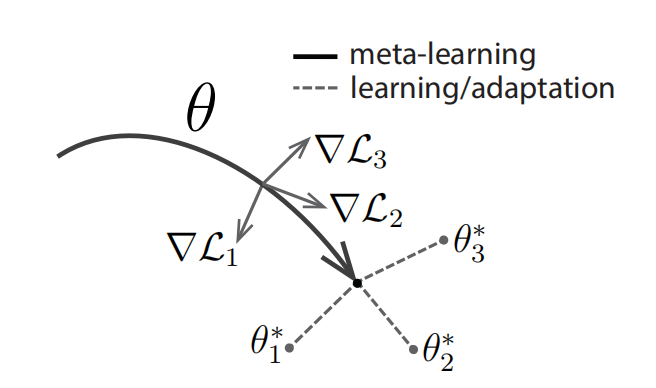
\includegraphics[totalheight=1.5in]{image/MAML.png}
  \caption{Diagram of our model-agnostic meta-learning algorithm (MAML)} \label{fig:graph}
\end{figure}

The gray branch lines in the figure represent the update direction of $\theta$ on different tasks, and the black line represents the final optimization of the model parameters, which can prevent the parameters from overfitting on a certain task. The last dotted lines represent processes of adaptation to new tasks, which is referred to as the fine-tune of the model parameters.

The gradient-based solution is adaptive to different kinds of learning tasks. Algorithm \ref{MAML} is the generalization of this model.



\begin{algorithm}[h]
  \caption{Model-Agnostic Meta-Learning}
  \label{MAML}
  \begin{algorithmic}[1]
    \REQUIRE $p(\mathcal{T})$: distribution over tasks
    \REQUIRE $\alpha, \beta$: step size hyperparameters
    \STATE randomly initialize $\theta$
    \WHILE {not done}
    \STATE Sample batch of tasks $\mathcal{T}_i \sim p(\mathcal{T})$
    \FORALL {$\mathcal{T}_i$}
    \STATE Evaluate $\nabla_\theta \mathcal{L}_{\mathcal{T}_i} (f_\theta)$ with respect to $K$ examples
    \STATE Compute adapted parameters with gradient descent: $\theta'_i = \theta - \alpha\nabla_\theta \mathcal{L}_{\mathcal{T}_i} (f_\theta)$
    \ENDFOR
    \STATE Update $\theta arrow \theta - \beta\nabla_\theta \Sigma_{\mathcal{T}_i \sim p(\mathcal{T})}\mathcal{L}_{\mathcal{T}_i} (f_{\theta'_i})$
    \ENDWHILE
  \end{algorithmic}
\end{algorithm}

At first, we sample several tasks randomly into a batch. From step 4 to step 7, we update the parameter vector $\theta'_i$ of the model separately on support set($D\_train$) of each task in the batch using one or more gradient descent updates on task $\mathcal{T}_i$.
While using multiple gradient updates is a straightforward extension, for simplicity of notation, we use one gradient update,
$$\theta'_i = \theta - \alpha\nabla_\theta \mathcal{L}_{\mathcal{T}_i} (f_\theta).$$
The step size $\alpha$ there can be a fixed hyperparameter or a meta-learned paramter. Loss function may be MSE in regression model or cross-entropy in classification.

After that, we need to compute the second gradient update, known as meta update, on the model parameters $\theta$ using the updated parameter vector $\theta'$. We no longer use the loss of each task to update the gradient, but like common model training process, optimizing for the performance of $f_{\theta'_i}$ with respect to $\theta$ across tasks sampled from
$p(\mathcal{T})$. More concretely, the meta-objective is as follows:
$$\min_\theta \Sigma_{\mathcal{T}_i \sim p(\mathcal{T})}\mathcal{L}_{\mathcal{T}_i} (f_{\theta'_i}) = \Sigma_{\mathcal{T}_i \sim p(\mathcal{T})}\mathcal{L}_{\mathcal{T}_i} (f_{\theta - \alpha\nabla_\theta \mathcal{L}_{\mathcal{T}_i} (f_\theta)})$$
The meta-optimization across tasks is performed via
stochastic gradient descent (SGD), such that the model parameters $\theta$ are updated as follows:
$$\theta arrow \theta - \beta\nabla_\theta \Sigma_{\mathcal{T}_i \sim p(\mathcal{T})}\mathcal{L}_{\mathcal{T}_i} (f_{\theta'_i})$$

The second gradient update is performed on the query set($D\_test$) in the task, which enhances the generalization of this model and avoids overfitting the support set($D\_train$).

% \begin{algorithm}
%   \caption{MAML for Few-Shot Supervised Learning}
%   \label{MAML}
%   \begin{algorithmic}[1]
%     \REQUIRE $p(\mathcal{T})$: distribution over tasks
%     \REQUIRE $\alpha, \beta$: step size hyperparameters
%     \STATE randomly initialize $\theta$
%     \WHILE {not done}
%     \STATE Sample batch of tasks $\mathcal{T}_i \sim p(\mathcal{T})$
%     \FORALL {$\mathcal{T}_i$}
%     \STATE Sample $K$ datapoints $\mathcal{D}=\{x^{(j)}, y^{(j)}\}$ from $\mathcal{T}_i$
%     \STATE Evaluate $\nabla_\theta \mathcal{L}_{\mathcal{T}_i} (f_\theta)$ with respect to $K$ examples
%     \STATE Compute adapted parameters with gradient descent: $\theta'_i = \theta - \alpha\nabla_\theta \mathcal{L}_{\mathcal{T}_i} (f_\theta)$
%     \STATE Sample datapoints $D'_i=\{x^{(j)}, y^{(j)}\}$ from $\mathcal{T}_i$ for the meta-update
%     \ENDFOR
%     \STATE Update $\theta arrow \theta - \beta\nabla_\theta \Sigma_{\mathcal{T}_i \sim p(\mathcal{T})}\mathcal{L}_{\mathcal{T}_i} (f_{\theta'_i})$
%     \ENDWHILE
%   \end{algorithmic}
% \end{algorithm}

\subsection{FOMAML}
MAML calculates the gradient twice in each iteration, which means that more calculation time is consumed. In response to this limitation, FOMAML, a variant of MAML, which avoids computing second derivative is proposed.

Our optimization goals in MAML are:
$$\operatorname{minimize}_{\theta} \mathbb{E}_{\tau}\left[L_{\tau}\left(U_{\tau}^{1}(\theta)\right)\right]$$
where $U_{\tau}^{k}(\theta)$ means to update the parameters $\theta$ using k samples of task $\tau$, so the gradient is:
$$g_{MAML}= \frac{\partial}{\partial \theta}\left[L_{\tau}\left(U_{\tau}^{1}(\theta)\right)\right]
  \\ = U_{\tau}^{1^{\prime}}(\theta) L_{\tau}^{\prime}\left(\theta_{\mathrm{new}}\right)
$$
Formula $U_{\tau}^{1^{\prime}}(\theta)=\frac{\partial}{\partial \theta}\left(\theta-\alpha \nabla_{\theta} L_{\tau_{i}}(\theta)\right)$ involves finding the second derivative, so it will be relatively time-consuming.

The method of FOMAML is not to find the secondary gradient, but instead of dividing into K different $\theta'_i$ when performing gradient calculation on K tasks, it uses the gradient calculated by the previous task in the gradient calculation of the next task. The final global gradient update also updates the parameter $\theta'_i$ obtained after calculating K tasks, and the gradient is:
$$
  g_{\mathrm{FOMAML}} =\frac{\partial}{\partial \theta_{i}}\left[L_{\tau}\left(U_{\tau}(\theta)\right)\right] \\
  =L_{\tau}^{\prime}\left(\theta_{i}\right).
$$


\subsection{Reptile}
Based on FOMAML, we introduce a new first-order gradient-based meta-learning algorithm called Reptile. Closely related to FOMAML, Reptile simply performs stochastic gradient descent (SGD) on each task in a standard way — it does not unroll a computation graph or calculate any second derivatives. This makes Reptile take less computation and memory than MAML. In global update, Reptile no longer calculates the gradient, but implements a soft way by using $\theta'_i$ to find $\theta$. The Reptile algorithm is as follows:

\begin{algorithm}[h]
  \caption{Reptile}
  \label{Reptile}
  \begin{algorithmic}[1]
    \STATE Initialize $\phi$, the vector of initial parameters
    \FOR {iteration = 1, 2, ...}
    \STATE Sample task $\tau$ , corresponding to loss $L_{\tau}$ on weight vectors $\widetilde{\phi} $
    \STATE Compute $\widetilde{\phi}=U_{\tau}^{k}(\phi)$, denoting k steps of SGD or Adam
    \STATE Update $\phi \leftarrow \phi+\epsilon(\widetilde{\phi}-\phi) $
    \ENDFOR
  \end{algorithmic}
\end{algorithm}

In the last step, we can treat $(\widetilde{\phi}-\phi)$ as a gradient and plug it into an adaptive algorithm such as Adam instead of simply updating $\phi$ in the direction $\widetilde{\phi}-\phi$.

We can also define a parallel or batch version of the algorithm that
evaluates on n tasks each iteration and updates the initialization to
$$\phi \leftarrow \phi + \epsilon \frac{1}{n} \sum_{i=1}^{n}\left(\widetilde{\phi}_{i}-\phi\right)$$

where $\widetilde{\phi}_{i}=U_{\tau_{i}}^{k}(\phi)$; the updated parameters on the $i^{th}$ task.
